\chapter{气井产气量预测算法}
在气井的全生命周期任务中,气井产量预测可以帮助企业有效规划气井的开发和生产过程,确定最佳的生产速率,以避免资源浪费和确保气井的长期稳定产出。同时,
准确的产气量预测有助于企业评估气井的经济价值,从而做出更加明智的投资决策,比如决定是否继续开发新的气田或是能呕对现有气井进行增产操作。过去比较广泛
的进行产量预测的方法是预测气井的绝对无阻流量,或者通过下降曲线分析的快速方法来匹配生产率-时间历史数据。但是这些现有的方法,在用于非常规储量估算的情况下,
有很多局限性且需要通过一些特定假设才能实现。这很难用于间歇生产气井产量预测,其会产生一些错误结果。本文采用时间序列预测的方式,目前油气产量时间序列预测的研究大多是同步
时间序列预测,应用场景有限。他们只是简单地将所有静态变量和动态变量直接连接在一起,忽略了特征之间的差异。基于这些痛点,本章根据
企业的专家经验设计了一种基于Transformer的气井产量预测算法,完成了气井产气量的时间序列预测任务。并根据企业的不同需要,又实现了基于LightGBM的产气量预测算法,让企业可以在进行预测任务时根据要求对算法选择。
\section{问题分析}
气井会因为它们的地理位置、地质构造、开采历史和技术等因素而表现出不同的产量特性。直接在所有气井数据上建立预测模型的话,模型就会过于复杂,难以捕捉到每一种类型气井的特点。而分类后,为每一类气
井建立模型可以简化问题,使得模型更容易泛化,减少过拟合的风险。本章将在第三章的基础上,根据不同的气井类别对气井进行时间序列预测。

在时间序列预测中,协变
量(covariates)是指与时间序列相关的其他变量。这些变量可以影响时间序列的行为和变化,因此在时间序列预测中使用协变量可以提高预测的准确性。
在本文的气井产气量预测问题中,使用协变量包括静态协变量(气井号WellNo,井丛号Cluster,集气站号Station),随时间变化的协变量
(Time-dependent Inputs),可以细分为过去可知,未来不可知的协变量(Past-observed Inputs),如井口压力\( \delta \)、套压\( \rho \)、
井口温度\( \sigma \)和日产量$\varphi $,以及过去和未来都可知的协变量
(Apriori-known Future Inputs),如如投产天数\( \tau \)、每日开井时间$h$等。此处,每日开井时间是一个影响产气量的重要因素,因为若开井时间为0,则产气量必定
为0。未来时刻的开关井时间受人工调控开关井的影响,是可知的,因此将其设置为过去和未来都可知的协变量。
\section{问题描述}
\subsection{单井产气量预测问题描述}
对于单个气井,其输入是气井一段时间的产量数据及对应的气井动态数据。对于单井一段时间内的数据,将其记为
\begin{equation}
    \left\{ (x_{\delta}^i, x_{\rho}^i, x_{\sigma}^i, x_{\tau}^i, x_{h}^i, y^i_{\varphi }) \mid i = 1, 2, \ldots, T \right\}
    \label{eq:singlewell}
\end{equation}
其中\( T \)表示气井数据的总时间长度,其中上标$i$表示时刻$i$,下标表示不同的特征,分别如下所示:井口压力\( \delta \)、套压\( \rho \)、
井口温度\( \sigma \)、投产天数\( \tau \)、每日开井时间$h$、日产量$\varphi $。则问题可以定义为:基于气井过去一段时间内的井口压力\( \delta \)等数据来预测气井未来一段时间内的产量,记要预测的未来时间步长$t$。形式化
地描述其输入如公式\eqref{eq:sinpredic}所示。
\begin{equation}
    \left\{
    \begin{array}{ll}
    (x_{\tau}^i, x_{\rho}^i, x_{\sigma}^i, x_{\tau}^i, x_{h}^i, y_{\varphi }^i) &  i = 1, 2, ..., T \\
    (x_{\tau}^{T+j}, x_{h}^{T+j}) & j = 1, 2, ..., t
    \end{array}
    \right.
    \label{eq:sinpredic}
\end{equation}    
输出为$\left\{ y^{T+1}_{\varphi}, y^{T+2}_{\varphi}, \ldots, y^{T+t}_{\varphi} \right\}$。

对于时序数据预测问题,需要将一整条数据依据时间点划分为训练数据和测试数据,然后需要设置训练数据步长与滑动步长,从而生成多个样本。因此为将问题转换为时间
序列问题,需设置新的符合并对问题作进一步地定义。记训练数据输入步长为$T$,$T$通常大于等于要预测的时间步长$t$,记滑动步长为$s$,记训练数据和测试数
据的划分时间点为$N_0$,记$\mathbf{X_i} = \{x^i_\delta, x^i_\rho, x^i_\sigma, x^i_\tau, x^i_h\}, \quad \mathbf{Y_i} = y^i_\varphi$,则训练数据可以用式\eqref{eq:traindata}表示。
\begin{equation}
    \begin{aligned}
    x_{\text{train}}^{(1)} &: \{ (X_1, Y_1), ..., (X_{T}, Y_{T}), (x^{T+1}_{\tau }, x^{T+1}_{h }), ..., (x^{T+t}_{\tau }, x^{T+t}_{h}) \}, \\
    y_{\text{train}}^{(1)} &: \{Y_{T+1}, ... ,Y_{T+t}\}, \\
    x_{\text{train}}^{(2)} &: \{ (X_{1+s}, Y_{1+s}), ..., (X_{T+s}, Y_{T+s}), (x^{T+s+1}_\tau , x^{T+s+1}_h ), ..., (x^{T+s+t}_{\tau }, x^{T+s+t}_{h}) \}, \\
    y_{\text{train}}^{(2)} &: \{Y_{T+s+1}, ... ,Y_{T+s+t}\}, \\
    & \vdots
    \end{aligned}
    \label{eq:traindata}
\end{equation}
测试数据可以用式\eqref{eq:testdata}来表示。
\begin{equation}
    \begin{aligned}
    x_{\text{test}}^{(1)} &: \{ (X_{N_0}, Y_{N_0}), ..., (X_{N_0 + T}, Y_{N_0 + T}), (x^{N_0 + T+1}_{\tau }, x^{N_0 + T+1}_{h }), ..., (x^{N_0 + T+t}_{\tau }, x^{N_0 + T+t}_{h}) \}, \\
    y_{\text{test}}^{(1)} &: \{Y_{N_0 + T+1}, ... ,Y_{N_0 + T+t}\}, \\
    & \vdots
    \end{aligned}
    \label{eq:testdata}
\end{equation}
最终,问题定义为构建机器学习/深度学习预测器$f_{ML }$,根据一段连续生产的历史数据预测未来时间长度$t$内的流量,即
\begin{equation}
    (Y_{n+1}, \ldots, Y_{n+t}) = f_{ML}(X_n, Y_n, X_{n-1}, Y_{n-1}, \ldots, X_{n-T+1}, Y_{n-T+1}, X^{n+1}_{\tau}, X^{n+1}_{h}, X^{n+t}_{\tau}, X^{n+t}_{h})
\end{equation}
    
\subsection{多井产气量预测问题描述}
现有产气量预测方法多为针对某一单一气井的建模,应用价值有限。每个气井的产量主控因素可能有较大差别,且很多参数是无法量化的,无法加入到机器学习中,带来了
较大的不确定性。因此,通过某一单一气井时间序列数据训练出的机器学习模型往往无法针对其他气井使用。

同时,对于本企业提供的气井数据集而言,一共包含1000余口气井的时间序列数据。一方面,要针对单一气井构建不同的时间序列模型是不现实的,单井的数据量是有限的,且部分气井仅具
有极少量数据,无法据此构建机器学习/深度学习模型,且模型过多会导致通用性差,难以管理等问题。另一方面,使用所有气井的数据集进行训练可以捕捉到不同气井之
间具有的相似的生产规律,可以提高模型的泛化性,实现对多气井产气量预测的统一建模。

本文的多气井产气量预测在单井产气量预测的基础上添加一系列静态协变量(包括气井号,井丛号和集气站号),并针对第三章得到的不同类别的气井生成特定类别的预测结果。因此多气井产量预测模型在
考虑了气井预测模型的泛化性的基础上又不失特殊性,从而实现了气井产量的高效预测。
\section{算法框架}
根据上文所述内容,需要根据气井的历史数据信息来预测气井的未来产量。本章具体的框架图如图\ref{fig:TFTprogess}所示。

本章提出的气井产量预测算法具体分为以下几个步骤:

(1)获取气井类别:根据第三章的方式对气井进行分类,以根据气井不同的类别分别进行预测。

(2)气井数据提取:本章使用企业提供的气井数据,并在第\ref{cha:data}章中对气井数据进行了数据清洗,使得其可以直接在接下来进行数据处理。

(3)气井数据预处理:使用滑动窗口对气井数据进行处理,接下来对数据进行无量纲化处理,将所有特征缩放至$[0,1]$之间。最终把得到数据集用于后续模型的训练、验证和测试。

(4)使用产气量预测算法分别对每类气井进行预测:根据企业的需要对选择合适的算法对产气量进行时间序列预测。
\begin{figure}[h]
    \centering
    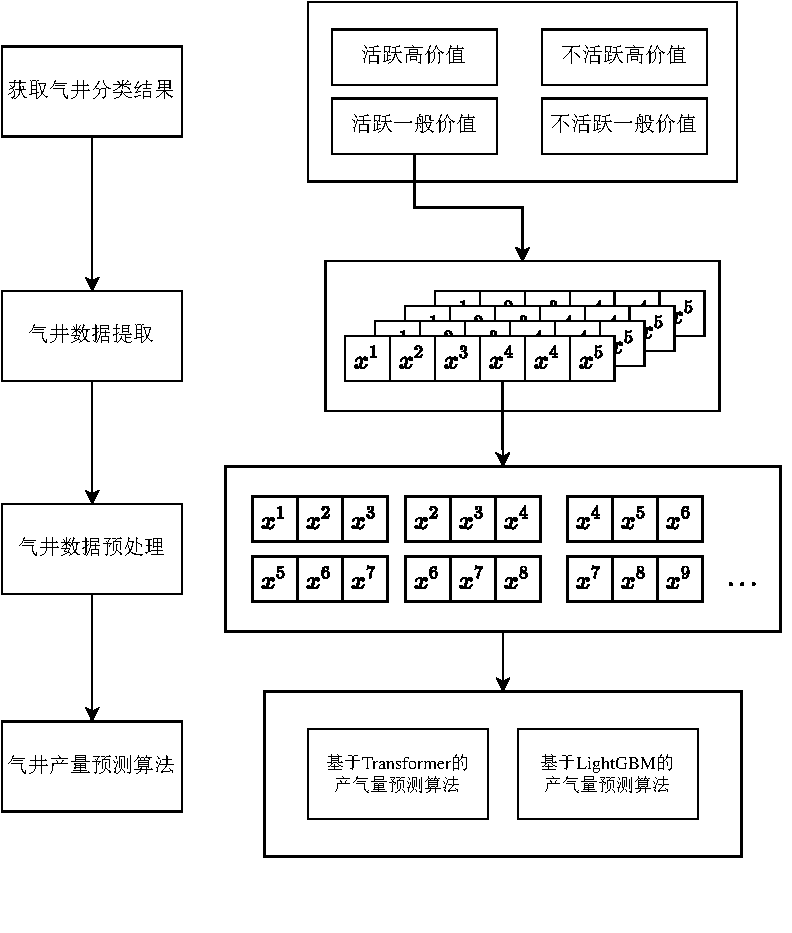
\includegraphics{figure/第四章框架图.vision.pdf}
    \caption{基于transformer的气井产量预测算法框架示意图}
    \label{fig:TFTprogess}
\end{figure}

\section{基于Transformer的气井产量预测算法}

\subsection{数据处理及分类}
\label{sec:datafoc}
气井的数据为第\ref{cha:data}章进行处理后的数据。

为了统一输入输出格式,
降低模型复杂度和计算开销,本文使用滑动窗口技术将
训练数据切割为固定长度。滑动窗口模式是进行序列预测问题处理的最常用的方式,通过控制窗口的大小,可以调整参与预测的历史数据的数量。其模型如
图\ref{fig:slidewindow}所示。
\begin{figure}[H]
    \centering
    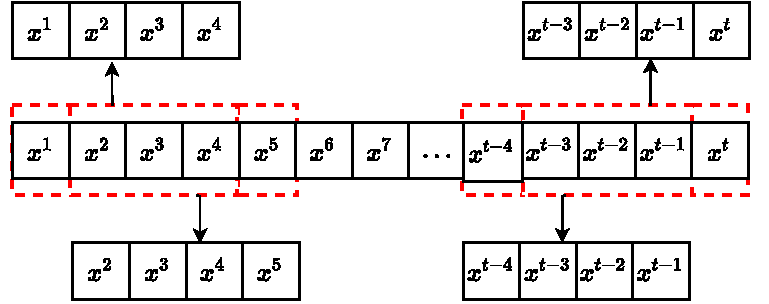
\includegraphics{figure/滑动窗口.vision.pdf}
    \caption{滑动窗口数据分段示意图}
    \label{fig:slidewindow}
\end{figure}
如图\ref{fig:slidewindow}所示,本文将预测步长设置为t, 将滑动窗口长度设置为$s$,用户在训练过程中,可以根据自己的需要对气井的时间序列进行划分。在取出样本序列后,每个样本分段的数据差异大且复杂,
未经标准化处理的样本分段会导致机器学习模型的学习速度十分缓慢,甚至无法更新模型参数,需要对每个样本分段进行无量纲化处理,将所有特征放缩至$[0,1]$之间,即
\begin{equation}
    x'_i = \frac{x_i - \mu}{\sigma}
\end{equation}
其中$x'_i$为标准化后的分段,$\mu$为该分段的均值,$\sigma$为该分段的标准差。
\subsection{算法主要设计策略}
如图\ref{fig:TFT}所示,为基于Transformer的气井产量预测算法的模型结构图。

本文借鉴了TFT对变量处理的思路,根据气井不同的协变量,将输入的历史时刻和未来时刻的特征经过一系列变换,得到一个抽象的
表征,然后分别输入到Encoder和Decoder中。Encoder部分使用GRU网络来编码历史时刻的信息,输出一个固定长度的向量,表示整个历史序列的含义。
Decoder部分使用自注意力机制来解码未来时刻的预测值,每个预测值都是根据之前所有时刻的加权结果得到的。

由于输入与目标之间的关系是未知的,对于预测结果而言,到底需要什么程度的非线性处理是一项巨大的挑战。非线性层过多会出现梯度消失或梯度爆炸的问题,因此,有时
需要简化模型来处理问题。为了让模型只在需要的时候才灵活地应用非线性地方式处理数据,本文采用了门控残差网络(GRN)来处理数据。

在时间序列的数据中,重要的点例如异常、变化点或者周期性模式一般都是根据他们周围的值来识别的。通过编码时间序列能够在序列中记忆和使用先前的信息,增强局
部上下文,从而提高基于注意力架构模型的性能。本文将采用时间特征处理层GRU来进行时间序列编码,
相较于LSTM,其具有更简单的结构,它合并了LSTM的遗忘门和输入门,因此参数数量较少,在训练和推理过程中的计算效率更高,且其有更快的训练速度,。在本文数据集规模较大的情况下进行实验和调整参数时更加高效。

在进行GRU编码后,本文采用自注意力来学习不同时间步之间的长期关系。最终借鉴MQRNN框架\cite{wen2018multihorizon}的思路,本文采用分位数回归预测作为模型的输出方式。

\begin{figure}[H]
    \centering
    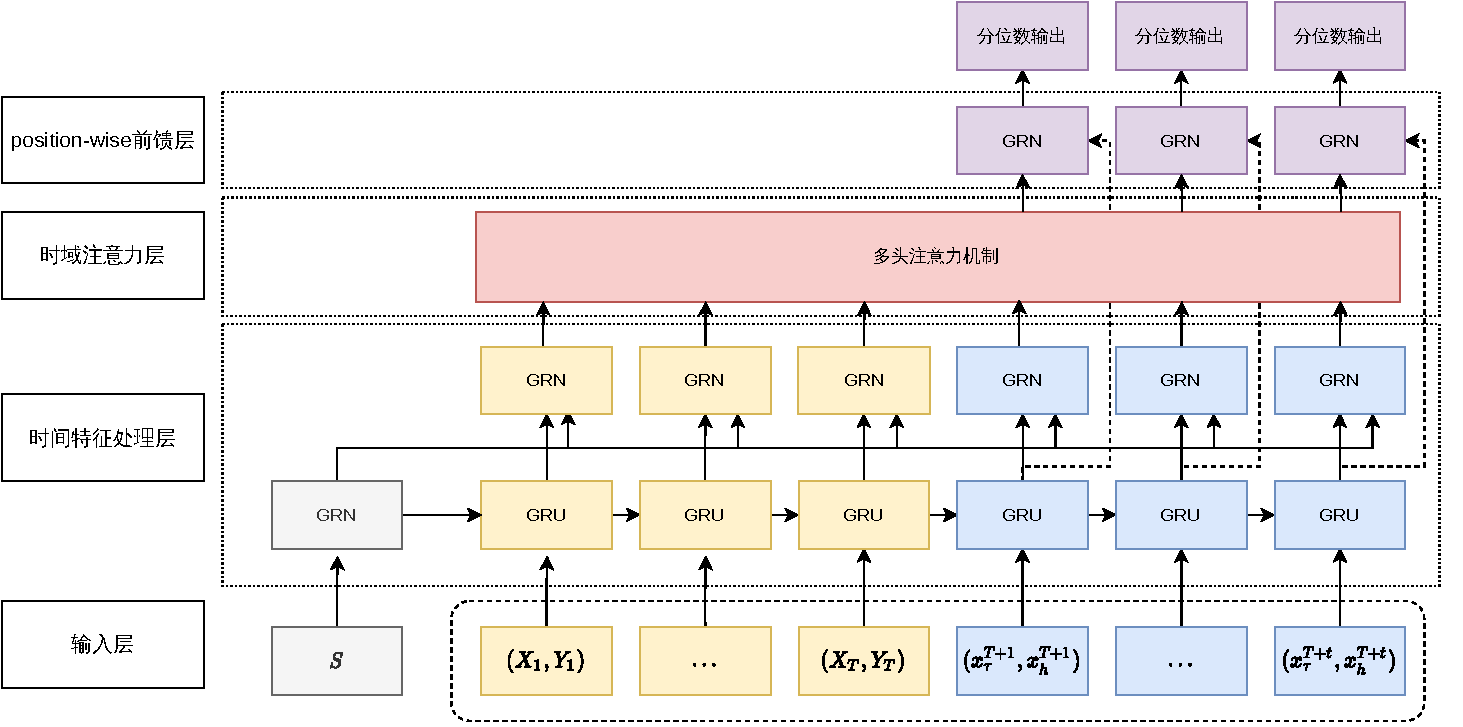
\includegraphics[width=.99\linewidth]{figure/基于Transformer的算法.vision.pdf}
    \caption{基于transformer的气井产量预测算法的模型结构图}
    \label{fig:TFT}
\end{figure}

综上所述,网络模型主要由门控残差网络、输入层、时间特征处理层、时域注意力层、position-wise前馈层以及分位数预测层组成具体如下:

(1) 输入层

本模型根据企业专家经验选取了多种数据并将他们融合。具体地由图中可知:输入层包括三种类型的变量。最左侧的$S$是静态变量,包括气井号$WellNO$、井丛号$cluster$和集气站号$Station$。从$(X_1, Y_1)$到$(X_{T}, Y_{T})$代表的是从过去时刻已知
,但未来不可知的随时间变化的变量,包括井口压力\( \delta \)、套压\( \rho \)、
井口温度\( \sigma \)和日产量$\varphi $。最右侧的$(x^{T+1}_{\tau }, x^{T+1}_{h })$到$(x^{T+t}_{\tau }, x^{T+t}_{h})$代表的是从过去$t-k$到未来$t+\tau_{max}$时刻
都可知的随时间变化的变量,包括已经如投产天数\( \tau \)、每日开井时间$h$等。

其中静态变量$S$需要经过静态协变量编码器来整合来自静态元数据的信息。具体地,本文使用上文采用的门控残差网络来编码产生上下文向量$\mathbf{c}_h$,$\mathbf{c}_e$
,$\mathbf{c}_h$将传入时间特征的局部处理层作为GRU的初始输入,$\mathbf{c}_e$可与进行时间特征编码后的动态变量一起进入GRN,流入多头注意力。

(2)门控残差网络

门控残差网络的输入为主输入$\mathbf{a}$
和一个可选的上下文向量$\mathbf{c}$。
其示意图如\ref{fig:GRN}所示。
\begin{figure}[H]
    \centering
    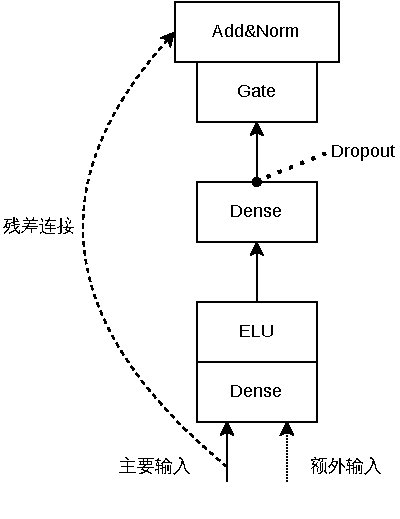
\includegraphics{figure/残差连接.vision.pdf}
    \caption{门控残差网络(GRN)示意图}
    \label{fig:GRN}
\end{figure}
具体操作如下所示:
\begin{equation}
    GRN_{\omega}(\mathbf{a}, \mathbf{c}) = \text{LayerNorm}(\mathbf{a} + GLU_{\omega}(\boldsymbol{\eta}_1))
\end{equation}
其中:
\begin{equation}
    \boldsymbol{\eta}_1 = \mathbf{W}_{1,\omega} \boldsymbol{\eta}_2 + \mathbf{b}_{1,\omega}
\end{equation}
\begin{equation}
    \boldsymbol{\eta}_2 = \text{ELU}(\mathbf{W}_{2,\omega} \mathbf{a} + \mathbf{W}_{3,\omega} \mathbf{c} + \mathbf{b}_{2,\omega})
    \label{eq:eta2}
\end{equation}
上式中,ELU是指线性激活函数,$\eta_1 \in \mathbb{R}^{d_{\text{model}}}$, $\eta_2 \in \mathbb{R}^{d_{\text{model}}}$ 是中间层,
LayerNorm是标准归一化,$\omega$ 是表示权重共享的索引。本文使用基于门控线性单元 (GLUs)的组件门控层来
控制非线性贡献的程度。假设 $\boldsymbol{\gamma } \in \mathbb{R}^{d_{\text{model}}}$ 是输入,GLU的形式为:
\begin{equation}
    GLU_{\omega}(\boldsymbol{\gamma }) = \sigma(\mathbf{W}_{4,\omega} \mathbf{\boldsymbol{\gamma }} + \mathbf{b}_{4,\omega}) \odot (\mathbf{W}_{5,\omega} \mathbf{\boldsymbol{\gamma }} + \mathbf{b}_{5,\omega}),
\end{equation}
其中 $\sigma(\cdot)$ 是sigmoid激活函数,$\mathbf{W}_{(\cdot)} \in \mathbb{R}^{d_{\text{model}} \times d_{\text{model}}}$ 是权重,$\mathbf{b}_{(\cdot)} \in \mathbb{R}^{d_{\text{model}}}$ 是偏置,
$\odot $ 是元素的Hadamard乘积。GLU允许模型控制GRN对原始输入$\mathbf{a}$的贡献程度:在必要的情况下,GLU的输出可以都接近于0,以便抑制模型非线性
的贡献。对于没有上下文向量$\mathbf{c}$的实例,GRN简单地将上下文输入视为0(即在\eqref{eq:eta2}中,$\mathbf{c}=0$)。

(3)局部时间特征处理

本文将过去的输入序列$\bm{\xi}_{1:T}$提供给编码器,将未来的输入序列$\bm{\xi}_{T+1:T+t}$
提供给解码器。使用GRU生成一组均匀的时间特征,作为下一阶段的输入,用$\phi (t,n)$来表示,
其中$\phi(t,n) \in {\phi(t, 1), \ldots, \phi(t, T+t)}$,$n$是位置指标。这种方式也可以完美处理观测到的过去和未来的输入不同而
存在的差异。同时,为了让静态数据也参与到时间序列变量的编码中,本文使用$\mathbf{c_h}$上下文向量初始化第一个GRU的隐藏状态。在此处也使用门控跳跃链接:
\begin{equation}
    \tilde{\bm{\phi}}(t, n) = \text{LayerNorm}\left(\tilde{\bm{\xi}}_{t+n} + \text{GLU}_{\phi}(\bm{\phi}(t, n))\right)
\end{equation}
其中$n \in [ -k, \tau_{\max}]$是位置指标。

为了让静态变量在模型中充分发挥作用,将静态变量和动态变量都经过GRN编码再送入时域注意力层,公式如\eqref{eq:staticencoder}层。
\begin{equation}
    \theta(t, n) = GRN_{\phi}(\hat{\phi}(t, n), c_e),
    \label{eq:staticencoder}
\end{equation}
其中$GRN_{\phi}$的权重在整个层中是共享的,$\mathbf{c}_e$是来自静态协变量得到的向量。

(4)时域注意力层

传统的多头注意力每个头使用不同的值,仅通过权重注意力本身并不能指示特定特征的重要性,此处
在传统多头注意力的基础上共享V。具体如下:
一般来说,注意力机制基于键矩阵\( K \in \mathbb{R}^{N \times d_{\text{attn}}} \)和查询矩阵\( Q \in \mathbb{R}^{N \times d_{\text{attn}}} \)
之间的关系对值\( V \in \mathbb{R}^{N \times d_v} \)进行缩放:
\begin{equation}
    \text{Attention}(Q, K, V) = A(Q,K)V
\end{equation}
其中$A()$是一个归一化函数,\( N \) 是进入注意力层的时间步数(即 \( k + t_{\text{max}} \))。常用的选择是缩放点积注意力:
\begin{equation}
    A(Q, K) = \text{Softmax}\left(\frac{QK^T}{\sqrt{d_{\text{attn}}}}\right)
\end{equation}
为了提高注意力机制的学习能力,Vaswani于2017年提出了多头注意力,使用不同的头针对不同的表示子空间:
\begin{equation}
    \text{MultiHead}(Q, K, V) = [H_1, \ldots, H_m]W_H
\end{equation}
\begin{equation}
    H_h = \text{Attention}(QW^Q_{(h)}, KW^K_{(h)}, VW^V_{(h)})
\end{equation}
其中\( W^K_{(h)} \in \mathbb{R}^{d_{\text{model}} \times d_{\text{attn}}} \), \( W^Q_{(h)} \in \mathbb{R}^{d_{\text{model}} \times d_{\text{attn}}} \), \( W^V_{(h)} \in \mathbb{R}^{d_{\text{model}} \times d_v} \) 
是针对键、查询和值的头特定权重 \( W_H \in \mathbb{R}^{m \cdot h \times d_{\text{model}}} \) 用于将所有头输出合并。
为了展示特定特征的重要性,做出的修改如下:
\begin{equation}
    \text{InterpretableMultiHead}(\mathbf{Q}, \mathbf{K}, \mathbf{V}) = \tilde{\mathbf{H}} \mathbf{W}_h
\end{equation}
\begin{equation}
    \begin{aligned}
        \mathbf{\tilde{H}} &= \tilde{A}(\mathbf{Q}, \mathbf{K}) \mathbf{V} \mathbf{W}_v, \\
        &= \left\{ \frac{1}{m_H} \sum_{h=1}^{m_H} A(\mathbf{Q} \mathbf{W}_Q^{(h)}, \mathbf{K} \mathbf{W}_K^{(h)}) \right\} \mathbf{V} \mathbf{W}_v, \\
        &= \frac{1}{m_H} \sum_{h=1}^{m_H} \text{Attention}(\mathbf{Q} \mathbf{W}_Q^{(h)}, \mathbf{K} \mathbf{W}_K^{(h)}, \mathbf{V} \mathbf{W}_v),
    \end{aligned}        
\end{equation}
式中:$\mathbf{W}_v \in \mathbb{R}^{d_{\text{model}} \times d_v}$是跨所有头共享的值的权重,$\mathbf{W}_h \in \mathbb{R}^{d_{\text{attn}} \times d_{\text{model}}}$
用于最终的线性映射。$\tilde{A}(\mathbf{Q}, \mathbf{K})$允许模型通过分析一组注意力权重来进行简单的可解释性研究。

在进行了时间特征处理层之后,需要应用注意力层。将所有的时间特征组合成单一的矩阵即$\bm{\varPhi }(t) = \left[ \bm{\theta} (t, -k), \ldots, \bm{theta }(t, \tau_{\text{max}}) \right]^T$
并在每个时间点($N = \tau _{max} + k + 1$)应用时域注意力:
\begin{equation}
    \mathbf{B}(t) = \text{InterpretableMultiHead}(\mathbf{\theta }(t), \mathbf{\theta }(t), \mathbf{\theta }(t)),
\end{equation}
生成了$\mathbf{B}(t) = \left[ \mathbf{\beta }(t, -k), \ldots, \mathbf{\beta }(t, \tau_{\max}) \right]$。在自注意力层之后,增加了一个额外
的门控层来促进训练:
\begin{equation}
    \boldsymbol{\delta}(t, n) = \text{LayerNorm}(\boldsymbol{\theta }(t, n)) + \text{GLU}_{\boldsymbol{\delta}}(\boldsymbol{\beta}(t, n)).
\end{equation}

(5)position-wise前馈层

对自注意力层应用额外的非线性处理,此处依然使用门控残差网络:
\begin{equation}
    \boldsymbol{\psi}(t, n) = \text{GRN}_{\boldsymbol{\psi}}(\boldsymbol{\delta}(t, n))
\end{equation}
其中$ \text{GRN}_{\boldsymbol{\psi}}$的权重在整个层中共享。此处还应用了一个跳过整个transformer块的残差连接,为序列到序列层提供了直接的路径。
倘若不需要额外的复杂性,就可以得到一个更简单的模型。如下所示:
\begin{equation}
    \tilde{\boldsymbol{\psi}}(t, n) = \text{LayerNorm}(\tilde{\boldsymbol{\delta}}(t, n)) + \text{GLU}_{\tilde{\boldsymbol{\psi}}}({\boldsymbol{\psi}}(t, n))
\end{equation}

\subsection{损失函数}

本文使用了分位数损失预测的方式。具体来说就是回归模型在对目标产量进行预测的时候不只预测$y$的一个期望值$\hat{y}$,
而是预测出$y$的概率分布中不同百分位数(如25\%,50\%,75\%)的值。分位数预测是根据上一步输出的线性变换生成的:
\begin{equation}
    \hat{\boldsymbol{y_i}}(q, t, \tau) = f_q (\tau, y_{i,1:T}, Z_{i,1:T}, X_{i,T:T+t}, S_i)
\end{equation}
其中,$\hat{\boldsymbol{y_i}}(q, t, \tau)$表示在时刻t,对未来$\tau$步进行预测的q分位数,$f_q(\cdot)$为预测模型,$ y_{i,1:T}$表示历史目标变量,$Z_{i,1:T}$表示过去已知,未来不可知的动态协变量,$X_{i,T:T+t}$表示过去未来都可知的动态协变量,$S_i$表示静态协变量。
本文采用联合最小化分位数损失来训练模型,并将所有的分位数方法相加,具体如式\eqref{eq:loss}所示。
\begin{equation}
    \mathcal{L}(\Omega, \mathbf{W}) = \sum_{y_t \in \Omega} \sum_{q \in \mathcal{Q} } \sum_{\tau=1}^{\tau_{\max}} \frac{\text{QL}(y_t, \hat{\boldsymbol{y}}(q, t - \tau, t), q)}{M_{\tau_{\max}}}
    \label{eq:loss}
\end{equation}
其中$\text{QL}(y,\hat{y},q)$为分位数损失,具体定义如下:
\begin{equation}
    \text{QL}(y, \hat{y}, q) = q(y - \hat{y})_+ + (1 - q)(\hat{y} - y)_+,
\end{equation}
在式\eqref{eq:loss}中,$\Omega$是包含M个样本的训练数据,$W$表示模型的权重,$\mathcal{Q}$是分位数的集合(用户可自行指定,本文使用$\mathcal{Q} = \{0.25,0.5,0.75\}$)。$\mathcal{L}(\Omega, \mathbf{W})$是平均单挑时序且平均预测点下的分位数损失。
由于$(\cdot)_+ = \max(0, \cdot)$,且$y-\hat{y}$与$\hat{y}-y$一定是一正一负,因此第二个公式可以转换为
\begin{equation}
    \text{QL}(y, \hat{y}, q) =  \max(q(y - \hat{y} ), (1 - q)(\hat{y} - y))
\end{equation}
假设拟合分位数0.75的目标值,代入公式即如式\eqref{eq:0.75}所示。
\begin{equation}
    \text{QL}(y, \hat{y}, q=0.75) =  \max(0.75(y - \hat{y} ), 0.25(\hat{y} - y))
    \label{eq:0.75}
\end{equation}
此时会有两种情况,若$(y - \hat{y} )$,即模型预测偏小,Loss增加会更多,否则模型预测偏大,Loss增加会更少。由于权重是3:1,所以训练时,模型会越来越趋向于预测出大的数字,这样Loss下降的更快,则模型的整个拟合的超平面会向上移动,
这样便能很好的拟合出目标变量的75分位数值。为了避免不同预测点下的预测量纲不一致问题,本文对随时函数进行了正则化处理。
\section{算法实现}
\subsection{基于transformer的气井产量预测算法}
为实现产气量预测算法,本文以XE9984-HI 气井数据为例,展示协变量的表示。如表\ref{tab:realdata}
所示,表分为上下两部分,具体每一列分别表示气井已经生产天数、集气站号、井丛好、气井号、配产量、日开井时间、井口压力、套压、井口温度、日产气量。得到气井数据后,需要先进行如章节\ref{sec:datafoc}所示的数据分段方法进行时间窗口的划分,由问题描述可知,训练样本可以表示为如式\eqref{eq:traindata}所示。
以预测未来45天的产气量为例,此时$t=45$,根据经验,T可以取值为75。气井数据表中完整的一行表示一对$(\mathbf{x_i},\mathbf{y_i})$,对于每次训练,其输入包括:$75 \times 5$(已经生产天数\( \tau \)、日开井时间h、井口压力\( \delta \)、套压\( \rho \)和
井口温度\( \sigma \)这五个动态变量) + $75 \times 3$(气井号WellNo,井丛号Cluster,集气站号Station这三个静态变量) + $45 \times 2$(如投产天数\( \tau \)、每日开井时间$h$这两个未来一直的动态变量)+ $75 \times 1$(历史产气量)。最终的输出为45维,表示未来45天的日产气量。
在模型训练阶段,使用前文的输入,未来45天的数据作为监督目标,进行模型训练。在推理阶段,使用上述输入生成未来时刻的预测结果。具体训练流程如\ref{al:T-GRU}所示,其中验证阶段是可选的。其中平均绝对误差MAE的计算公式为$MAE = \frac{1}{n} \sum_{i=1}^{n} |y_i - \hat{y}_i|$
\begin{table}
    \caption{XE9984-HI气井数据示例}
    \label{tab:realdata}
    \begin{tblr}{hlines,vlines,
        columns = {valign=m,co=-1},
        rows    = {halign=c},}
        Elapsed Production & Station & Cluster & WellNO & Allocation \\
        362 & FF & 99 & XE9984-HI & 1.0000 \\
        362 & FF & 99 & XE9984-HI & 1.0000 \\
        362 & FF & 99 & XE9984-HI & 1.0000 \\
        362 & FF & 99 & XE9984-HI & 1.0000 \\ 
        362 & FF & 99 & XE9984-HI & 1.0000 \\ 
        DailyHour & WellHead Pressure & CasingHead Pressure & WellHead Temperature & Daily Production  \\
        24.0000 &3.0800 &0.0000 &6.5100 &0.2666  \\
        24.0000 &3.0300 &0.0000 &3.5300 &0.3460  \\
        24.0000 &3.0600 &0.0000 &5.0800 &0.3176  \\
        24.0000 &3.0500 &0.0000 &6.8400 &0.5038  \\
        24.0000 & 3.0200&0.0000 &6.1600 &0.4473  \\
    \end{tblr}
\end{table}

\begin{algorithm}[H]
    \baselineskip=20pt
    \caption{基于Transformer的气井产量预测算法训练过程}
    \label{al:T-GRU}
    \begin{algorithmic}[1]
    \Require 滑动窗口后的训练数据集$X_{train}$和验证数据集$X_{valid}$
    \Ensure 得到合适参数的模型M

    \For{ i $\in$ epochs}
        \State 初始化train\_mae为空
        \For{ j $\in$ $X_{train}$}
            \State 清除旧的梯度避免梯度累计
            \State 前向传播得到产气量结果$y_{train}$
            \State 与实际产气量结果根据式\ref{eq:loss}计算损失
            \State 根据损失进行反向传播
            \State 更新模型参数
        \EndFor    
        \State 计算并记录MAE损失
        \State 调整学习率

        \State 初始化valid\_mae为空
        \For{j $\in$ $X_{valid}$}
            \State 不计算梯度
            \State 前向传播得到得到产气量结果$y_{valid}$
            \State 计算并记录MAE损失
        \EndFor
        \State 计算验证集的平均mae损失
    \EndFor
    \end{algorithmic}
  \end{algorithm}
\subsection{基于LightGBM的气井预测算法}
根据前文所述,本问题需要同时对1000余口气井构建时间序列预测模型,且问题包含多种类型的协变量,由第一章的国内外研究现状可知,机器学习模型中,当前对于时间序列预测问题的主流选择是特征工程+LightGBM模型的方法,这也是当前各大时间序列竞赛中大多数获胜方案所采用的策略。
下面将对LightGBM模型的设计做具体介绍。

决策树模型可以用于回归预测任务,其基本原理是将输入变量空间划分成多个子空间,并在每个子空间内拟合一个简单的回归模型。在预测时,将输入数据映射到对应的子空间,并用该子空间内的回归模型来进行预测,从而得到最终的预测结果。

集成树模型的原理是将多个弱学习器(例如决策树)组合成一个强学习器,从而提高预测的准确性和稳定性。在具体的实现中,集成树模型通常采用Bagging或Boosting的方法进行集成。其中Boosting是一种迭代式的方法,通过序列化训练多个决策树模型,每次训练的模型都会针对前一轮的错误进行优化,从而逐步提升模型的准确性。在Boosting中,还有一种著名的算法叫做梯度提升树(Gradient Boosting Tree),它通过在每轮迭代中拟合负梯度来进行模型训练。LightGBM(Light Gradient Boosting Machine)是一种基于决策树的梯度提升框架,是由微软亚洲研究院开发的。它具有高效性和准确性,尤其适用于处理大规模数据集。相较于其他梯度提升框架,LightGBM 在训练速度和内存使用方面具有优势。

多步时间序列预测是指根据历史数据来预测未来多个时刻的数据,例如预测未来一周的天气或销量。要使LightGBM模型适应于多步时间序列预测,需要进行以下几个步骤:

数据准备:对于本问题,需要将历史产气量数据按照气井号和时间顺序进行排序,并且将数据集划分为训练集,验证集和测试集。同时,需要对静态协变量和随时间变化的协变量进行特征工程处理。
数据准备过程分为数据清洗和数据划分,数据清洗如\ref{cha:data}所述,数据划分部分选取每口井最后一段forecast horizon长度的气井产量数据作为测试集(forecast horizon指要预测的长度,如对未来45天的每日产气量进行
预测),选取倒数第二个forecast horizon长度的气井产量数据作为验证集,验证集用来调整lightGBM模型的超参数,其余数据用作测试集。

对时间序列数据进行特征工程,抽取延迟特征、滑动窗口特征等。在该问题中,所选取的静态特征包括,集气站号Station,井丛号Cluster,气井号WellNo,配产量Allocation,其余特征包括表示时间的整数Elapsed,这个整数值通过当前日
期与数据集第一天的日期差计算得到,表示气井生产时长的整数值ElapsedProduction,通过当前日期与气井投产日期的日期差计算得到,当日开井时间DailyHour,延迟特征Lag1到Lag30,其中延迟特征Lagi表示当前日期前i天的产气量,即使
用过去的产气量数据预测未来产气量(这里以预测未来7天的产气量为例,使用过去30天的数据预测未来7天的产气量),滑动特征RollingMean7,RollingStd7,……,RollingMean180, RollingStd180,其中RollingMeani和RollingStdi分
别表示过去i天产气量数据的均值和方差,i取{7,15,30,60,180},通过Rolling特征提取历史产气量数据的数值信息。这里具体使用过去多长时间的历史数据对未来进行预测通常根据经验选取,通常这个长度在forecast horizon到2*forecast horizon之间。
进行特征工程后,构造训练数据,将每个时刻的产气量作为目标值和对应的特征作为一条样本,具体如表\ref{tab:asamplefeature}所示。
\begin{table}[H]
    \renewcommand{\arraystretch}{1.5}
    \centering
    \caption{一条样本所包含的特征}
    \label{tab:asamplefeature}
    \begin{tblr}{hlines, vlines,
        columns = {valign=m,co=-1},
        rows    = {halign=c},}
        名称 & 集气站号 & 井丛号 & 气井号 & 配产量 & 所有时间长度 \\
        特征 & Station & Cluster & WellNo & Allocation & Elapsed \\
        名称 & 投产时长 & 当日开井时间 & 前i天产气量 & 均值滑动特征 & 方差滑动特征\\
        特征 &Elapsed Production & DailyHour & Lag{i} & RollingMean{i} & RollingStd{i}\\
    \end{tblr}
\end{table}
表\ref{tab:singlesamp}表示一条训练样本(再加上进行特征工程Lag和Rolling特征),DailyProduction表示当日产气量是目标值。
\begin{table}[H]
    \renewcommand{\arraystretch}{1.5}
    \centering
    \caption{单条样本示意表}
    \label{tab:singlesamp}
    \begin{tblr}{hlines, vlines,
        columns = {valign=m,co=-1},
        rows    = {halign=c},}
        Station & Cluster & WellNO & Elapsed \\
        X5 & 997 & XE2213-HU9 & 1 \\
        ElapsedProduction &Allocation & DailyHour & DailyProduction \\
        1& 10.0000 & 3.60000 & 1.40000 \\
    \end{tblr}
    % \begin{tabular}{|c|c|c|c|}
    %     \hline
    %     Station & Cluster & WellNO & Elapsed \\
    %     \hline
    %     X5 & 997 & XE2213-HU9 & 1 \\
    %     \hline
    %     ElapsedProduction &Allocation & DailyHour & DailyProduction \\
    %     \hline
    %     1& 10.0000 & 3.60000 & 1.40000 \\
    %     \hline
    % \end{tabular}
\end{table}
调整LightGBM模型的参数,根据不同
的目标函数、评价指标、学习率、树的深度、叶子节点数等进行手动或自动调优。最终模型选择超参数如表\ref{tab:LightGBMSuper}所示,使用huber损失函数,MAE作为指标来对模型预测效果拟合效果进行评价。
\begin{table}[H]
    \renewcommand{\arraystretch}{1.5}
    \centering
    \caption{基于LightGBM的气井预测算法超参数}
    \label{tab:LightGBMSuper}
    \begin{tblr}{hlines, vlines,
        columns = {valign=m,co=-1},
        rows    = {halign=c},}
        Name & boosting type & objective & metric & min data in leaf & max depth & subsample \\
        Value & gbdt & huber & mae & 20 &8 & 0.8 \\
        Name & colsample bytree & learning rate & max bin & n estimators & boost from average & verbose \\
        Value & 0.8 & 0.05 & 1000 & 3000 & True & -1 \\
    \end{tblr}
    % \begin{tabular}{|c|c|c|c|c|c|c|}
    %     \hline
    %     Name & boosting\_type & objective & metric & min\_data\_in\_leaf & max\_depth & subsample \\
    %     \hline
    %     Value & gbdt & huber & mae & 20 &8 & 0.8 \\
    %     \hline
    %     Name & colsample\_bytree & learning\_rate & max\_bin & n\_estimators & boost\_from\_average & verbose \\
    %     \hline
    %     Value & 0.8 & 0.05 & 1000 & 3000 & True & -1 \\
    %     \hline
    % \end{tabular}
\end{table}
其中huber损失函数的定义如式\eqref{eq:huber}所示。
\begin{equation}
    L_{\delta}(y, f(x)) = 
        \begin{cases} 
        \frac{1}{2}(y - f(x))^2, & \text{if } |y - f(x)| \leq \delta \\
        \delta|y - f(x)| - \frac{1}{2}\delta^2, & \text{if } |y - f(x)| > \delta
        \end{cases}
    \label{eq:huber}
\end{equation}
在中,\(f(x)\)为预测值,δ为Huber损失函数的参数,δ接近0时,
Huber损失趋向于MAE。δ越大时,Huber损失趋向于MSE,在梯度下降时 MSE较MAE更为准确。而在异常值出现时 MAE较MSE更加鲁棒。Huber损失函数集中了两者的优势。这里MAE损失的定义如式\eqref{eq:Maeloss}所示。
\begin{equation}
    MAE = |y - f(x)|
    \label{eq:Maeloss}
\end{equation}

MSE损失的定义如式\eqref{eq:mseloss}所示。
\begin{equation}
    MSE = (y - f(x))^2
    \label{eq:mseloss}
\end{equation}

确定训练样本和模型超参数后,即可进行LightGBM模型的训练过程。在推理阶段,使用训练好的模型对于任一指定气井未来一段时间内的单日产气量做出预测。

在训练好的模型中,通过递归预测的方式,预测未来若干天的产气量。具体地,从当前时刻开始,先用模型预测未来第一天的产气量,然后将预测结果作为已知量(未来第二天地Lag1特征)输入到模型中,再预测未来第二天的产气量,以此类推。

\section{本章小节}
本章介绍了对气井产气量预测的必要性,并根据时间序列数据协变量的特征将气井的变量进行分类,定义了气井产气量预测的数学模型,并提出了一种基于transformer的气井产气量预测算法,并描述了其实现细节。同时为了应对企业的不同需求,本章对本文算法以及基于lightGBM的气井预测算法都进行了实现,可供企业在产气量预测时进行多样化选择。
